\chapter{Validation et résultats}

\section{Introduction}

Ce chapitre présente la validation fonctionnelle de la plateforme \textbf{Virtual FabLab}, les résultats obtenus, ainsi que les limites actuelles du travail réalisé. Après la description de l'implémentation dans le chapitre précédent, il s'agit ici de vérifier que les principales fonctionnalités répondent aux besoins définis : consultation du laboratoire virtuel, gestion des machines, réservation, simulation 3D, authentification, administration et communication entre le frontend et le backend.

La validation effectuée reste adaptée au contexte d'un projet de fin d'études. Elle porte principalement sur le bon fonctionnement des parcours utilisateurs et administrateurs, ainsi que sur la cohérence des échanges entre les différentes couches de l'application. Les parties liées à l'IoT et à la Data Science sont abordées avec prudence, car elles reposent encore sur des données simulées ou sur une base préparée pour une intégration future avec des équipements réels.

\section{Validation fonctionnelle de la plateforme}

\subsection{Tests du frontend}

Les tests du frontend ont porté sur les interfaces développées avec Next.js. L'objectif était de vérifier que les pages principales sont accessibles, lisibles et cohérentes avec les rôles des utilisateurs. Les interfaces testées incluent notamment la page d'accueil, le laboratoire 3D, la page des machines, les réservations, le tableau de bord administrateur et les pages de gestion.

La navigation a également été vérifiée afin de s'assurer que l'utilisateur peut passer d'un module à l'autre sans rupture de parcours. Les redirections vers la page de connexion sont déclenchées lorsque l'utilisateur n'est pas authentifié, tandis que les pages réservées à l'administrateur restent protégées pour les utilisateurs étudiants.

La partie simulation 3D a été validée à travers le chargement de la scène du FabLab, la sélection des machines et la visualisation des actions associées. Les modules de simulation CNC et imprimante 3D ont été testés avec des fichiers de démonstration afin de vérifier l'affichage des trajectoires, la progression de la simulation et la gestion des fichiers non valides. Ces tests confirment le caractère opérationnel de la simulation dans un objectif pédagogique, même si elle ne reproduit pas encore l'ensemble des phénomènes physiques réels.

\subsection{Tests du backend FastAPI}

La validation du backend FastAPI a concerné l'authentification, les routes protégées, les API REST et la gestion des erreurs. Le mécanisme d'authentification repose sur un jeton JWT généré lors de la connexion. Ce jeton permet ensuite d'accéder aux routes protégées selon le rôle de l'utilisateur.

Les tests effectués ont permis de vérifier les comportements suivants :

\begin{itemize}
    \item création d'un compte utilisateur avec des données valides ;
    \item connexion et récupération du jeton JWT ;
    \item accès au profil de l'utilisateur connecté ;
    \item protection des routes nécessitant une authentification ;
    \item restriction des routes administrateur aux utilisateurs autorisés ;
    \item création, consultation et traitement des réservations ;
    \item consultation et gestion des machines selon les permissions.
\end{itemize}

La validation des requêtes a également été prise en compte. Lorsque les données envoyées sont incorrectes ou incomplètes, le backend retourne des erreurs adaptées. Les principaux cas traités concernent les erreurs d'authentification, les accès interdits, les ressources inexistantes et les conflits liés aux réservations. Cette gestion permet au frontend d'afficher des messages compréhensibles et d'éviter les comportements incohérents.

\subsection{Communication frontend/backend}

La communication entre le frontend et le backend est centralisée dans la fonction utilitaire \texttt{apiRequest}. Cette fonction joue un rôle important dans l'organisation du code, car elle évite de répéter la logique d'appel API dans chaque page ou composant.

Son rôle consiste principalement à construire l'URL du backend, ajouter les en-têtes nécessaires aux échanges JSON, intégrer le token JWT lorsqu'il est disponible, puis traiter les réponses retournées par le backend. Lorsqu'une erreur HTTP est renvoyée, la fonction récupère le message d'erreur et le transforme en information exploitable par l'interface.

\begin{figure}[H]
\centering
\IfFileExists{images/api_communication.png}
{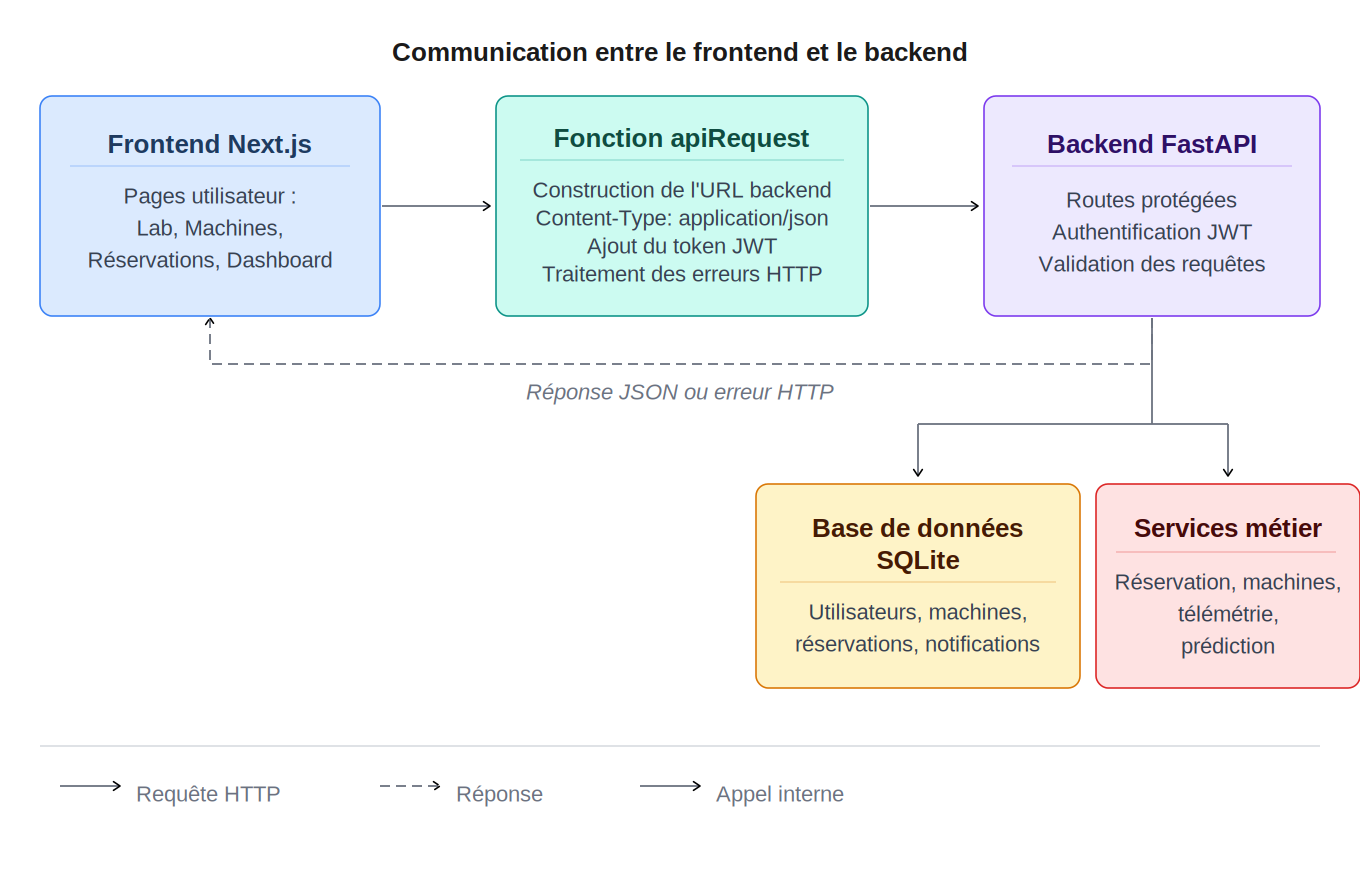
\includegraphics[width=0.9\textwidth]{images/api_communication.png}}
{\fbox{\parbox[c][5cm][c]{0.85\textwidth}{\centering Emplacement réservé pour le schéma de communication frontend/backend\\\texttt{images/api\_communication.png}}}}
\caption{Schéma de communication entre l'interface Next.js et le backend FastAPI}
\label{fig:api-communication-validation}
\end{figure}

La figure \ref{fig:api-communication-validation} illustre le principe général des échanges. Le frontend envoie une requête HTTP vers l'API FastAPI. Le backend valide la requête, applique la logique métier, interagit avec la base de données ou les services concernés, puis retourne une réponse JSON ou une erreur HTTP. Cette organisation rend la communication plus claire et facilite l'évolution de la plateforme.

\section{Résultats obtenus}

Les résultats obtenus montrent que la plateforme développée constitue un prototype fonctionnel répondant aux objectifs principaux du projet. L'application web permet à l'utilisateur de consulter les machines, accéder au laboratoire virtuel, effectuer des réservations et visualiser des simulations liées aux machines numériques.

Du côté administrateur, la plateforme permet la gestion des machines, des utilisateurs et des réservations. La séparation entre le frontend Next.js et le backend FastAPI rend l'architecture plus claire et facilite la maintenance du projet. Les routes backend assurent la persistance des données, la sécurité et l'exposition des fonctionnalités sous forme d'API REST.

La simulation 3D est opérationnelle pour représenter le FabLab virtuel et illustrer le comportement de machines telles que la CNC et l'imprimante 3D. Elle apporte une dimension visuelle et pédagogique importante au projet, en permettant à l'utilisateur d'interagir avec les machines avant une utilisation réelle.

Enfin, le projet fournit une base solide pour l'intégration future de l'IoT et de la Data Science. Les mécanismes liés à la télémétrie, à la supervision et à l'analyse de données sont préparés ou simulés, ce qui permet de démontrer l'orientation du système vers un FabLab connecté et intelligent sans prétendre à une validation industrielle complète.

\section{Limites actuelles et perspectives}

Malgré les résultats obtenus, certaines limites doivent être mentionnées. La première concerne la télémétrie, qui reste simulée. Les données utilisées permettent de tester les flux et les interfaces, mais elles ne remplacent pas des mesures réelles issues de capteurs installés sur des machines physiques.

La deuxième limite concerne l'absence de connexion directe avec de vraies machines IoT. Les scénarios de communication MQTT et de supervision sont préparés, mais ils nécessitent encore une validation avec des équipements réels. De même, la simulation 3D ne reproduit pas totalement le comportement réel des machines, notamment les contraintes mécaniques, les vibrations, les variations thermiques ou les défauts de fabrication.

Plusieurs perspectives peuvent être envisagées pour améliorer la plateforme :

\begin{itemize}
    \item intégrer un broker MQTT réel et des messages provenant de machines physiques ;
    \item ajouter des capteurs IoT pour collecter des mesures de température, vibration ou vitesse ;
    \item enrichir la maintenance prédictive à partir de données historiques réelles ;
    \item améliorer le réalisme de la simulation CNC et imprimante 3D ;
    \item développer un dashboard analytique plus avancé avec des courbes, alertes et indicateurs de performance.
\end{itemize}

Ces perspectives montrent que la solution actuelle peut servir de base évolutive. Elle permet déjà de valider l'architecture et les principaux parcours fonctionnels, tout en laissant une marge d'amélioration importante vers une plateforme plus connectée et plus intelligente.

\section{Conclusion}

Ce chapitre a présenté la validation fonctionnelle de la plateforme, les résultats obtenus ainsi que les limites actuelles du projet. Les tests réalisés confirment le fonctionnement des principaux modules : frontend, backend, authentification, gestion des machines, réservations, simulation 3D et communication API.

La plateforme Virtual FabLab répond ainsi aux objectifs essentiels du projet, tout en restant réaliste sur les limites liées à la simulation et à l'absence de machines IoT réelles. Elle constitue une base fonctionnelle et évolutive pour de futurs travaux autour de la supervision, de l'analyse de données et de la maintenance prédictive dans un FabLab connecté.
